\pdfminorversion=7
\pdfinfoomitdate=1
\pdftrailerid{}
\pdfsuppressptexinfo=-1
\documentclass[11pt]{article}

\usepackage[T1]{fontenc}
\usepackage[utf8]{inputenc}
\usepackage[margin=1in]{geometry}
\usepackage{amsmath,amssymb,amsthm}
\usepackage{booktabs}
\usepackage{graphicx}
\usepackage{float}
\usepackage{microtype}
\usepackage{xcolor}
\usepackage{hyperref}
\usepackage{url}

\hypersetup{
  colorlinks=true,
  linkcolor=blue!55!black,
  citecolor=blue!55!black,
  urlcolor=blue!55!black,
  pdftitle={Tolerance-aware auditing and a rational interval certificate for variable-radius circle packing},
  pdfauthor={Juan Jose Fernandez Morales}
}

\newtheorem{theorem}{Theorem}
\newtheorem{proposition}{Proposition}
\newcommand{\R}{\mathbb{R}}
\newcommand{\tauzero}{\tau=0}

\title{Tolerance-aware auditing and a rational interval certificate\\
for a variable-radius circle packing with 26 circles}
\author{Juan Jos\'e Fern\'andez Morales\\
\small G\"other Labs\\
\small \href{https://github.com/juan-fernandez-gotherlabs/circle-packing-tolerance-audit}{Reproducibility repository}}
\date{August 9, 2026}

\begin{document}

\maketitle

\begin{abstract}
We study the problem of placing 26 circles of independently variable radii in
the unit square while maximizing the sum of their radii.  Public numerical
results for this problem are often reported under different feasibility
tolerances, so their objective values are not directly comparable.  We provide
three separate finite-decimal certificates for the contracts
$\tau=10^{-6}$, $10^{-10}$, and $0$, together with an exact-rational verifier
and a hash-authenticated acquisition of public witnesses.  Each author
certificate ranks first among the complete acquired witnesses valid under its
matching rational contract.  More importantly, we give a computer-assisted
proof for the real 78-contact configuration near the strict finite-decimal
witness.  Exact rational interval arithmetic proves
a strict Krawczyk inclusion for the 78 active polynomial gap equations,
strict feasibility of all 351 inactive geometric constraints, and a second
Krawczyk inclusion for the Karush--Kuhn--Tucker multipliers.  All 78
multipliers are positive.  The active gaps are therefore local coordinates,
and the configuration is a strict local maximizer.  The argument uses only the
Python standard library on its verification path.  This is a local theorem and
a reproducibility result, not a proof of global optimality or a new packing
record.
\end{abstract}

\section{Introduction}

For centers $(x_i,y_i)$ and radii $r_i>0$, $0\leq i<26$, consider
\begin{equation}
  \max \; f(x)=\sum_{i=0}^{25} r_i                                      \label{eq:objective}
\end{equation}
subject to containment in $[0,1]^2$ and pairwise non-overlap.  The problem is
an instance of variable-radius circle packing, with 78 continuous variables
and 429 geometric inequalities.  It is nonconvex and admits many contact
topologies.

Computational reports can become misleading when a higher objective value is
obtained by consuming a larger feasibility tolerance.  A value accepted at
$10^{-6}$ cannot fairly be ranked against a strict feasible witness without
recording the two contracts.  Our first contribution is therefore
methodological: finite-decimal data are interpreted as exact rational numbers,
and every public witness is evaluated separately under a named tolerance.

Our main mathematical result concerns the 78-contact real root near the strict
finite-decimal witness.  We certify a unique regular root in a rational box of
radius $10^{-90}$ and enclose a positive vector of KKT multipliers.  This
converts numerical evidence of stationarity into a rigorous proof of strict
local optimality.

Interval methods have a substantial history in packing.  Mark\'ot used
interval arithmetic to establish structural optimality for congruent-circle
packings in the unit square \cite{markot2007}, and interval techniques also
appear in the broader computational treatment of square packings
\cite{szabo2007}.  We do not claim that interval certification of circle
packing is new in itself.  The contribution here is the explicit rational,
independently executable certificate for this variable-radius, sum-of-radii
configuration, combined with tolerance-aware public-corpus auditing.

The complete reproducibility artifact is archived at Zenodo
\cite{artifact}; the repository cited in Section~\ref{sec:repro} contains the
matching certificate and reports.  The public numerical table currently
attributes the $n=26$ value to Haowei Lin \cite{packomania}; consequently, no
new geometry or Packomania record is claimed.

\paragraph{Contributions.}
\begin{enumerate}
  \item We formalize three non-interchangeable feasibility contracts and
  publish a standard-library exact-rational verifier for the associated
  finite-decimal witnesses.
  \item We provide a reproducible, hash-authenticated acquisition and
  same-tolerance evaluation of complete public witnesses from an explicit
  corpus.
  \item We prove that the unique real solution of a specified 78-contact
  system in a rational interval box is a strict local maximizer of
  \eqref{eq:objective}.
\end{enumerate}

\section{Problem and numerical contracts}                              \label{sec:model}

Write
\[
  x=(x_0,y_0,r_0,\ldots,x_{25},y_{25},r_{25})\in\R^{78}.
\]
For each circle define its four wall gaps
\[
  x_i-r_i,\quad 1-x_i-r_i,\quad y_i-r_i,\quad 1-y_i-r_i,
\]
and, for $i<j$, the squared pair gap
\begin{equation}
  q_{ij}(x)=(x_i-x_j)^2+(y_i-y_j)^2-(r_i+r_j)^2.             \label{eq:pairgap}
\end{equation}
At zero tolerance, feasibility is equivalent to nonnegative wall gaps,
$q_{ij}\geq0$, and positive radii.

For a rational tolerance $\tau\geq0$, the repository contract permits wall
gaps of at least $-\tau$ and requires
\begin{equation}
 (x_i-x_j)^2+(y_i-y_j)^2\geq(r_i+r_j-\tau)^2                 \label{eq:tolerance}
\end{equation}
whenever $r_i+r_j-\tau>0$.  All decisions are made over the rational numbers;
square roots are used only to print diagnostic margins.  This linear-distance
allowance is not asserted to reproduce every upstream binary64 decision at a
rounding boundary.  Source-native binary64 evaluators are reimplemented and
reported separately when available.

Table~\ref{tab:contracts} gives the three primary certificates.  The two
relaxed witnesses fail when rechecked at zero tolerance, while the last row is
a strict feasible rational lower bound.

\begin{table}[ht]
\centering
\caption{Primary finite-decimal certificates.  Scores in different rows are
not interchangeable because the feasibility contracts differ.}
\label{tab:contracts}
\begin{tabular}{@{}lll@{}}
\toprule
Contract & Exact-rational recomputed score & Interpretation \\
\midrule
$10^{-6}$  & $2.63599872089287514$ & relaxed linear-distance contract \\
$10^{-10}$ & $2.63598308647338795$ & stricter relaxed contract \\
$0$        & $2.63598308491760778318\ldots$ & strict rational witness \\
\bottomrule
\end{tabular}
\end{table}

Each primary verification makes 429 geometric decisions and 26 radius
positivity decisions.  The strict witness was obtained by rounding a
high-precision contact root to 90 decimal places and conservatively reducing
all radii by approximately $10^{-75}$.  Thus the serialized CSV is exactly
feasible but is not itself the boundary root certified below.

\begin{figure}[H]
  \centering
  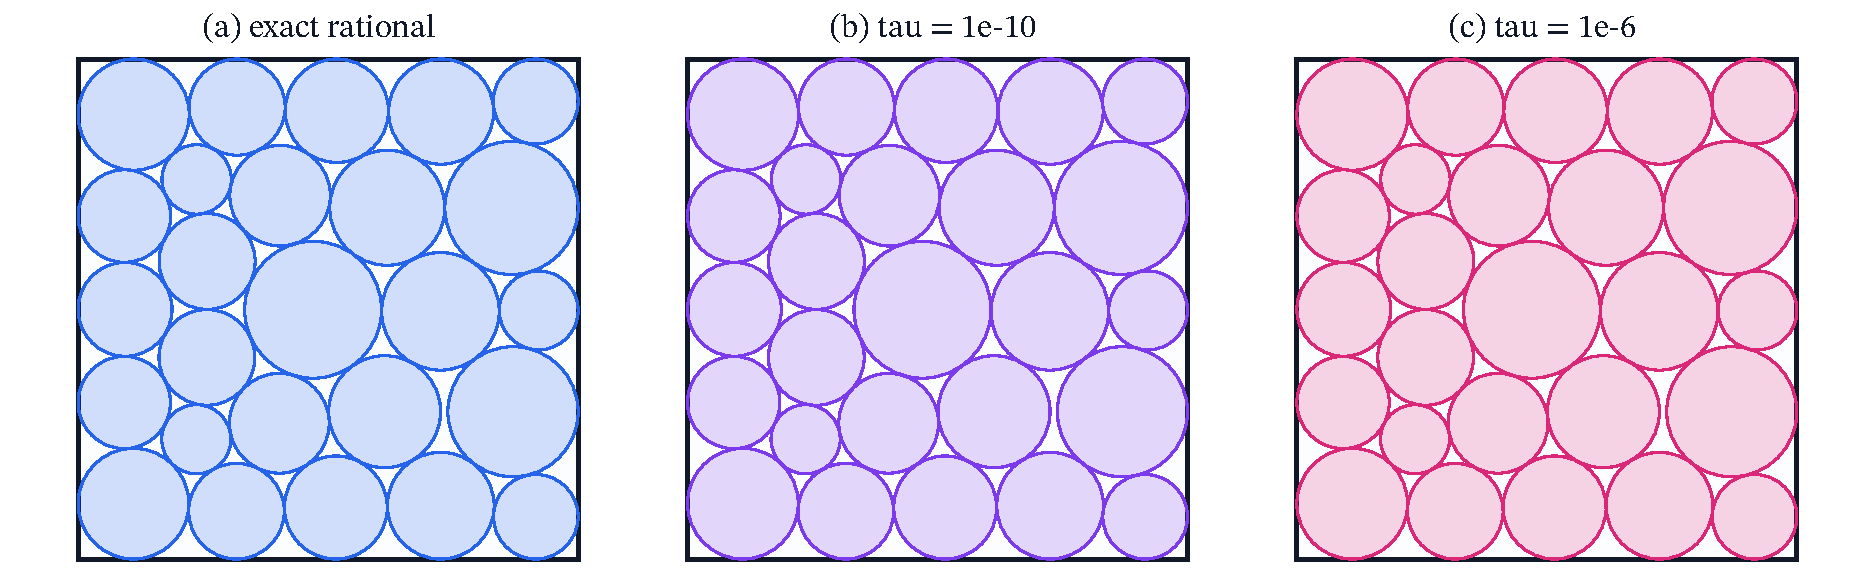
\includegraphics[width=\textwidth]{../figures/tolerance_certificates.pdf}
  \caption{The three serialized witnesses, kept separate by feasibility
  contract and shown at one common scale.  Their geometric differences and
  tolerance-scale violations are smaller than the plotted line width; a
  picture therefore cannot replace the contract-aware verifier.  The relaxed
  witnesses consume their stated tolerance and fail at zero tolerance.}
  \label{fig:tolerance-layouts}
\end{figure}

\section{Reproducible public-corpus audit}                              \label{sec:audit}

The source manifest pins immutable Git artifacts by full commit identifier and
SHA-256.  Downloaded Python files and notebooks are parsed as data and are
never imported or executed.  Numeric tokens are retained as decimal strings
before conversion to rational numbers.  The Packomania text file is not
available through an immutable URL; its observed payload is hash-pinned and a
changed download makes the default acquisition fail closed.

At the snapshot date, nine upstream artifacts were authenticated and ten
complete witnesses were evaluated.  Figure~\ref{fig:tolerance-rankings}
reports the five leading valid witnesses under each rational contract; the
complete tables, validity matrix, hashes, and exclusions are generated in the
archived artifact.  Exactly one matching author certificate is included in
each panel, and the author's certificates for the other contracts are
excluded.

The tolerance labels are audit contracts applied by this work, not
necessarily categories declared by the upstream projects.  Every complete
serialized witness was re-evaluated under all three contracts, and panel
membership is determined solely by the resulting exact-rational validity and
score.  In particular, the Packomania decimal is not treated as an entry
originally submitted at $\tau=10^{-10}$: its serialized value misses strict
feasibility by approximately $1.04\times10^{-12}$ and therefore first becomes
admissible in our $10^{-10}$ panel.  Conversely, AlphaEvolve v2 passes the
reconstructed native binary64 zero-tolerance evaluator but misses our
exact-rational zero contract by approximately $5.23\times10^{-17}$, a
rounding-boundary distinction.

Under an independent reimplementation of the EurekAgent native binary64
evaluator with $\mathrm{atol}=10^{-6}$, the matching author witness scores
$2.635998720892875$ and the public EurekAgent witness scores
$2.6359987208598832$.  This is a source-contract comparison inside the
manifested corpus, not a universal rank.  AlphaZ-CORAL was authenticated but
excluded because its public file computes radii at runtime rather than
serializing a complete witness.  Numaro and HELIX were recorded as reported
claims because no complete downloadable $n=26$ witness was located during the
snapshot.

The three panels make the comparison contract-local.  Every row in a panel
passes the same exact-rational feasibility test, so its position and score may
be compared with the other rows in that panel.  Positions must not be compared
across panels because the feasible sets differ.

\begin{figure}[H]
  \centering
  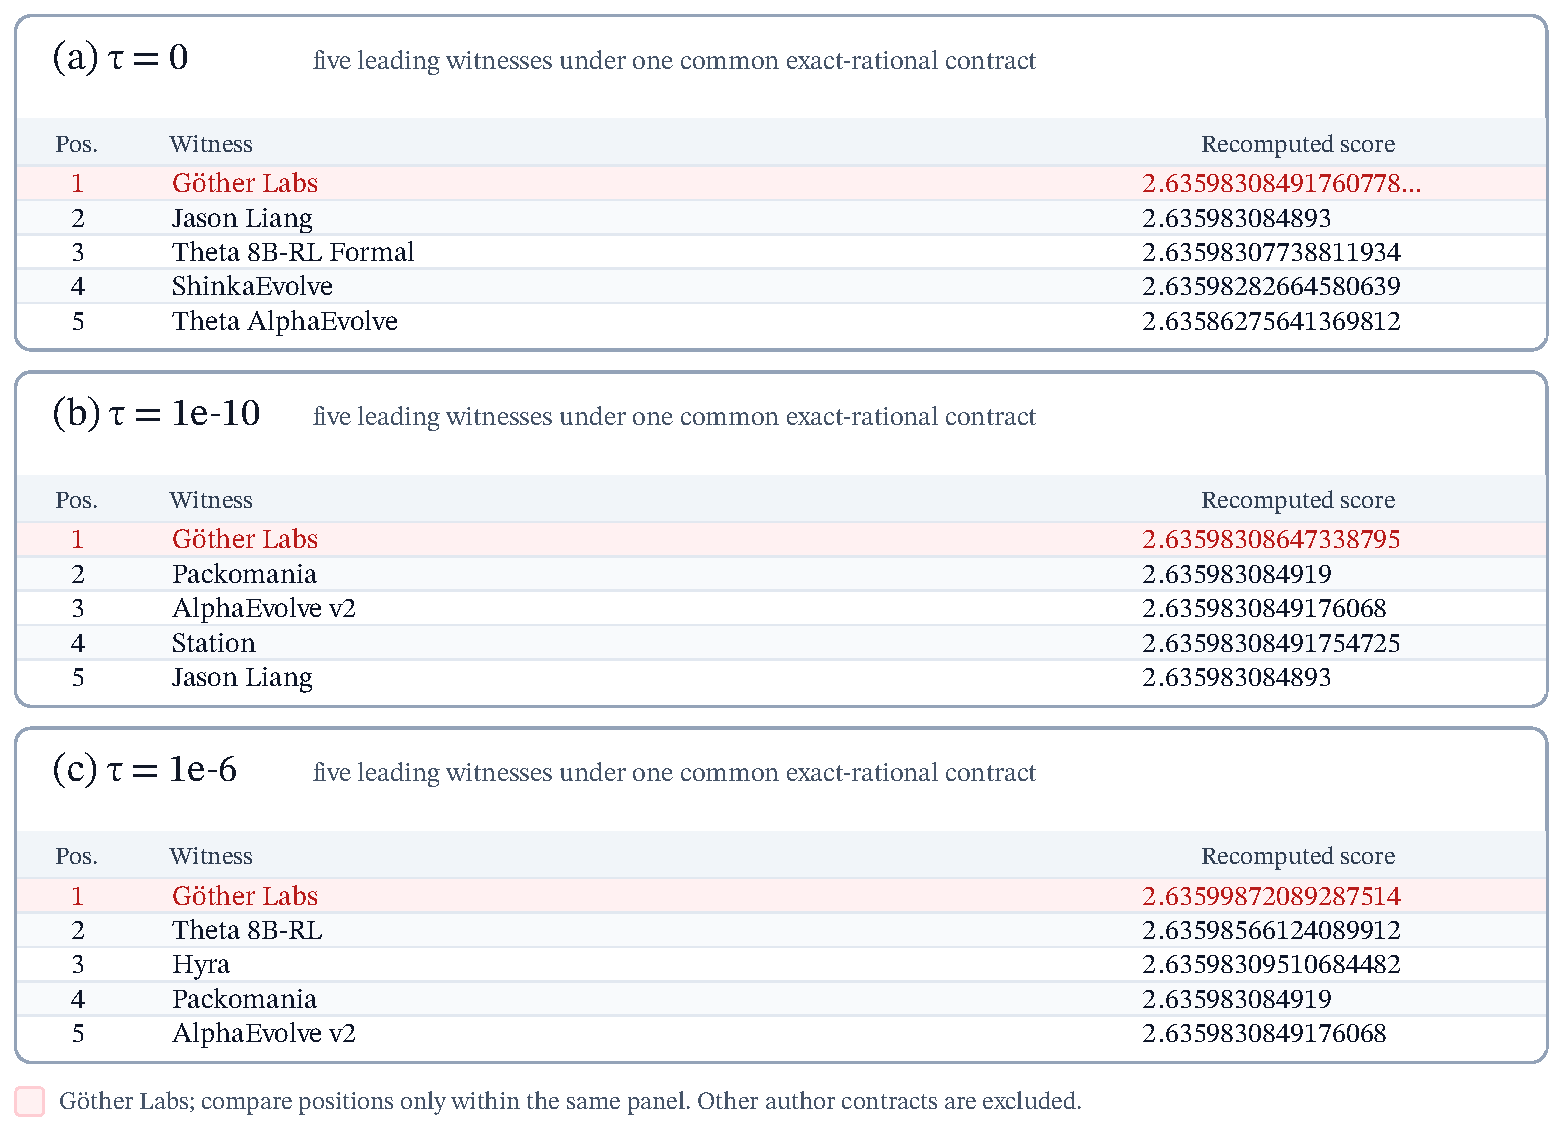
\includegraphics[width=\textwidth]{../figures/tolerance_rankings.pdf}
  \caption{Tolerance-separated positions in the explicitly manifested corpus.
  Each panel contains the five leading complete witnesses valid under one
  common exact-rational contract.  The highlighted G\"other Labs row is the
  only author certificate in its panel.  Scores are aligned at the decimal
  point; ellipses truncate displayed digits only.  Panel positions are not
  universal leaderboard claims and are not compared across tolerances.  Panel
  membership reflects our re-evaluation, not an upstream tolerance
  designation.}
  \label{fig:tolerance-rankings}
\end{figure}

Within this deliberately bounded corpus it is accurate to describe each
matching author certificate as the \emph{best exact-rationally re-evaluated
witness in the manifested corpus}.  The unqualified phrase ``best-known'' would be
stronger than the evidence: the corpus is not exhaustive, and reported claims
without complete downloadable witnesses cannot be independently ranked.

\section{The active polynomial system}                                 \label{sec:system}

The strict witness identifies 78 active constraints: 58 circle--circle
contacts and 20 wall contacts.  Let
\[
  g:\R^{78}\longrightarrow\R^{78}
\]
collect the corresponding wall gaps and squared pair gaps.  Since wall gaps
are affine and \eqref{eq:pairgap} is quadratic, $g$ is polynomial and its
Jacobian $J=Dg$ is affine.  This avoids transcendental interval extensions.

The proof certificate stores a rational midpoint $m$, a rational box
$X=m+[-\rho,\rho]^{78}$ with $\rho=10^{-90}$, and rational preconditioners.
For a preconditioner $C$, the interval Krawczyk image is
\begin{equation}
 K(X)=m-Cg(m)+(I-CJ(X))(X-m).                                \label{eq:krawczyk}
\end{equation}
All interval endpoints and all acceptance comparisons are computed using
arbitrary-size integers and rational fractions.  Floating-point libraries are
used only by an optional certificate-generation mode; they do not participate
in verification.

The exact computation gives
\begin{align}
 K(X)&\subset\operatorname{int}(X),                                      \label{eq:incl}\\
 \max_k\frac{\sup|K_k(X)-m_k|}{\rho}
     &<8.551052960068879\times10^{-15},                                  \label{eq:ratio}\\
 \lVert I-CJ(X)\rVert_\infty
     &<8.551052960068879\times10^{-15}.                                  \label{eq:norm}
\end{align}
The Krawczyk theorem \cite{krawczyk1969} therefore gives a unique zero
$x^*\in X$.  The norm bound also proves that every Jacobian represented in the
box is nonsingular.  Direct rational interval evaluation proves that all 351
inactive geometric gaps are strict and all radii are positive:
\begin{align}
 \min(\text{inactive polynomial gaps})&>
 0.0071877548062774697881043072924253371679,                 \label{eq:inactive}\\
 \min_i r_i&>
 0.0691806763572344820974407544002623682677.                 \label{eq:radii}
\end{align}

\section{Dual certificate and strict local optimality}                 \label{sec:proof}

Use the convention that feasible gaps satisfy $g\geq0$.  Stationarity for the
maximization problem is
\begin{equation}
  \nabla f(x^*)+J(x^*)^T\lambda=0.                           \label{eq:kkt}
\end{equation}
A second rational Krawczyk test encloses the solution of this interval linear
system in a dual box of radius $10^{-10}$.  Its maximum component inclusion
ratio is below $7.677651441669678\times10^{-6}$, and
\begin{equation}
  \min_k\lambda_k>0.020825602106288.                         \label{eq:lambda}
\end{equation}

\begin{theorem}[Certified strict local maximum]                         \label{thm:main}
The unique zero $x^*$ of the named 78-contact system in $X$ is a strictly
feasible packing with respect to every inactive constraint and is a strict
local maximizer of $f=\sum_i r_i$ over all feasible packings of 26
variable-radius circles in the unit square.
\end{theorem}

\begin{proof}
Equations \eqref{eq:incl}--\eqref{eq:norm} prove existence, uniqueness, and
nonsingularity of $J(x^*)$.  Equations \eqref{eq:inactive} and
\eqref{eq:radii} show that the enclosed root is a packing and that no inactive
constraint becomes active at the root.

By the inverse function theorem, $z=g(x)$ is a system of local coordinates in
a neighborhood of $x^*$.  Restrict the coordinate image, if necessary, to a
convex ball about $0$, and set $F(z)=f(g^{-1}(z))$.  From
\eqref{eq:kkt},
\[
  \nabla_zF(0)=J(x^*)^{-T}\nabla f(x^*)=-\lambda.
\]
Every component is strictly negative by \eqref{eq:lambda}.  By continuity,
after shrinking the coordinate neighborhood if necessary, every component of
$\nabla_zF$ remains negative.  Any nearby feasible packing has $z\geq0$;
if it differs from $x^*$, then $z\neq0$.  Integrating along the segment from
$0$ to $z$ yields
\[
 F(z)-F(0)=\int_0^1\nabla F(tz)\mathbin{\cdot}z\,dt<0.
\]
The inactive constraints remain strict in a sufficiently small neighborhood,
so this covers all nearby feasible packings.  Hence $x^*$ is a strict local
maximizer.
\end{proof}

No Hessian test is required: the active gradients form a basis and the
critical cone is trivial.  Approximate numerical rank and multiplier signs
alone would not justify the theorem; the primal and dual interval inclusions
are essential.

The certified score interval at the contact root implies the more compact
outward-rounded enclosure
\[
\begin{aligned}
f(x^*)&>2.6359830849176077831865694854434817303966767982744,\\
f(x^*)&<2.6359830849176077831865694854434817303966767982745.
\end{aligned}
\]
The substantially longer rational endpoints are retained in the
machine-readable report.  The root score is slightly above the deliberately
shrunken finite-decimal witness.

\section{Reproducibility}                                               \label{sec:repro}

The principal proof can be rerun from the repository root with
\begin{verbatim}
python3 -S scripts/prove_local_optimum.py
\end{verbatim}
where \texttt{-S} disables third-party site packages.  The command parses all
certificate decimals as rational numbers, verifies the primal and dual
inclusions, and regenerates the JSON proof report.  The full audit, tests,
table generation, and visualization run with
\begin{verbatim}
./verify_all.sh
\end{verbatim}
The public corpus can be refreshed online or replayed from an authenticated
cache.  Third-party programs are never executed.  The artifact records the
reference software environment, hashes, upstream commits, source licenses,
and the provenance boundary of private exploratory material.

The contact graph in Figure~\ref{fig:packing} is generated from the strict
certificate.  It contains 58 pair contacts and 20 wall contacts.

\begin{figure}[H]
  \centering
  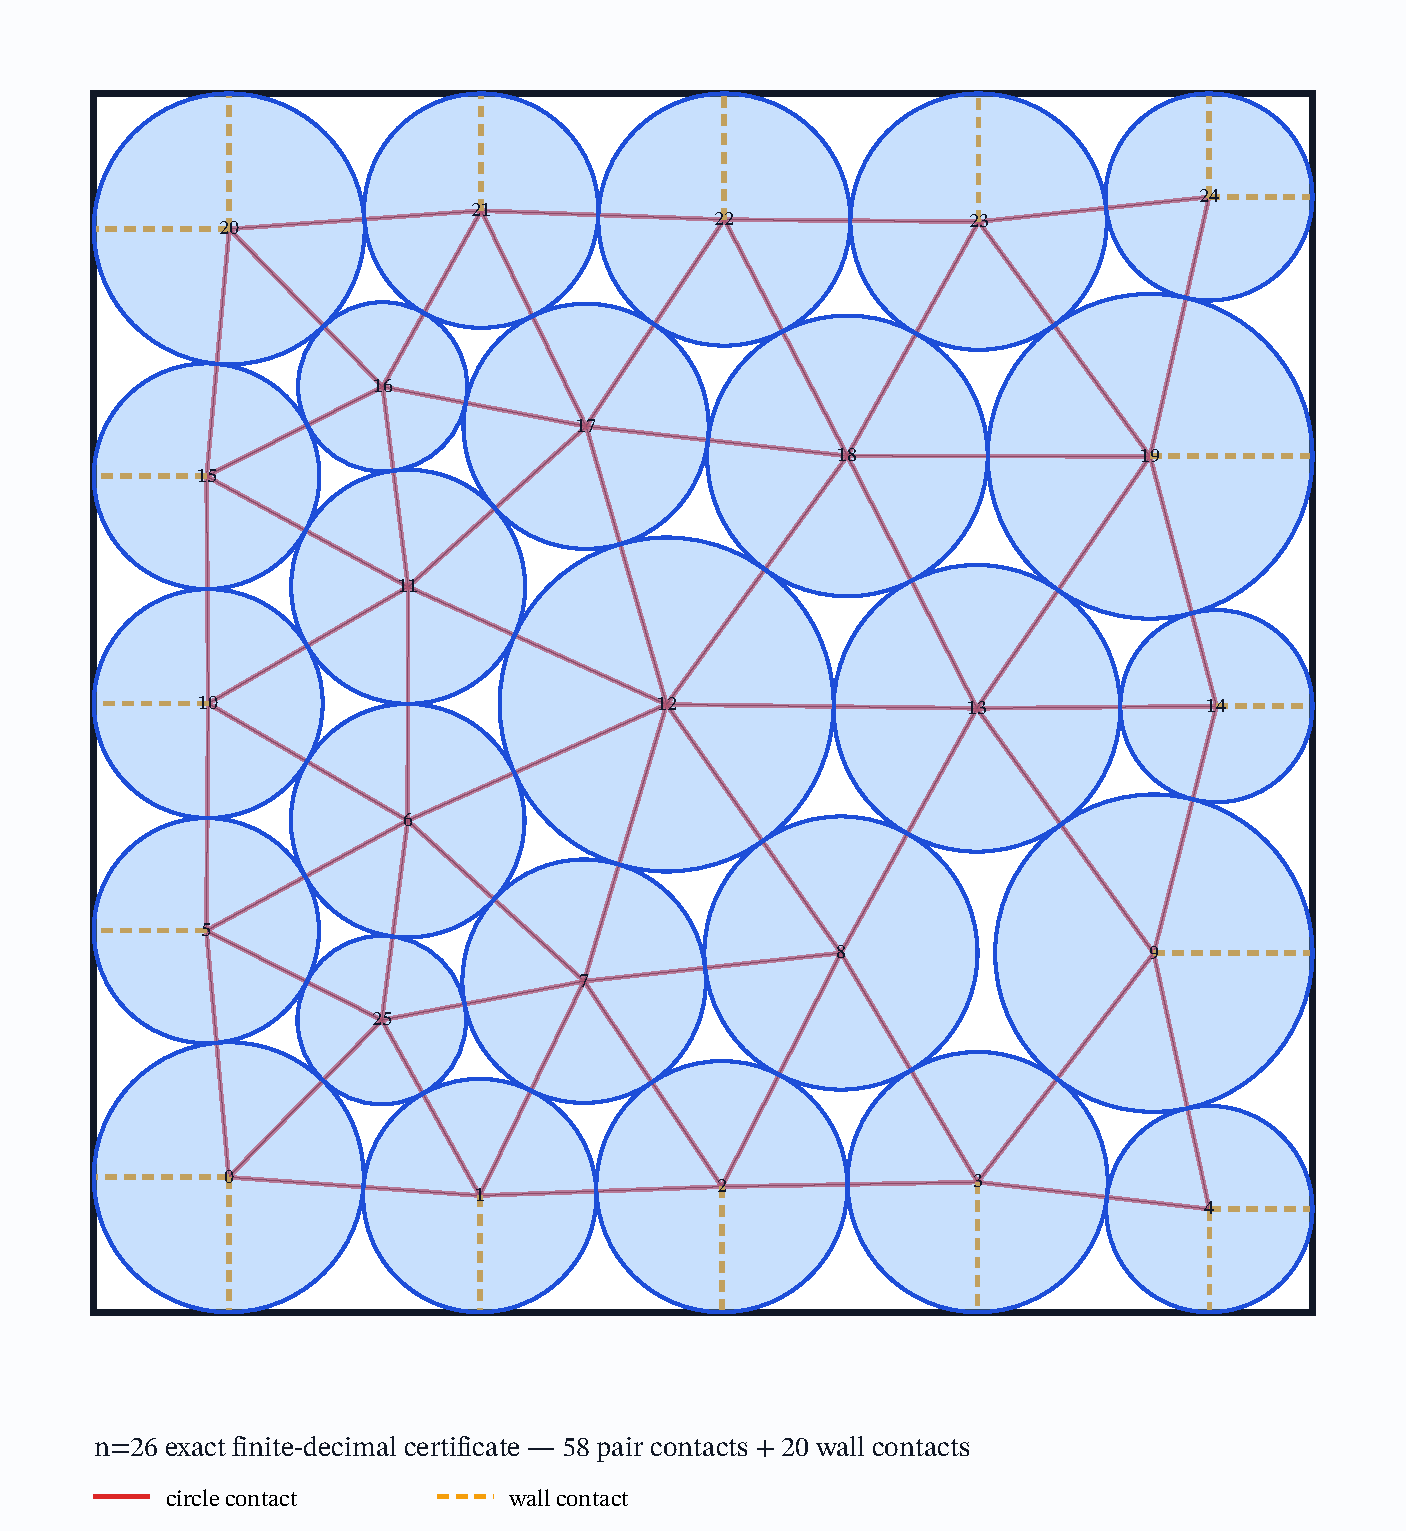
\includegraphics[width=0.76\textwidth]{../figures/exact_packing_contact_graph.pdf}
  \caption{The 26-circle strict witness and its reconstructed contact graph.
  The interval theorem concerns the nearby exact real contact root.}
  \label{fig:packing}
\end{figure}

\section{Scope and limitations}

Theorem~\ref{thm:main} is deliberately local.  It neither supplies a global
upper bound nor rules out a superior packing with a different contact graph.
The configuration was already public, and its score agrees with the current
public $n=26$ value to the displayed precision; we claim neither a new record
nor discovery of a new layout.  The public-corpus positions cover only the
explicit, hash-manifested sources and exclude claims lacking complete
downloadable witnesses.  Scores belonging to different tolerance contracts
must not be compared as if they shared one feasible set.

The method also certifies only one contact root.  Applying the same verifier to
several values of $n$ or several contact topologies would be needed to support
a broader methodological claim.  A separate implementation in another
interval package would provide useful defense in depth, although the present
proof path is already independent of binary floating-point acceptance
decisions.

\section{Conclusion}

Separating numerical contracts resolves an ambiguity that otherwise rewards
larger constraint violations with larger apparent objective values.  For the
strict $n=26$ configuration, exact rational interval computation goes further:
it certifies a unique regular contact root, strict inactive feasibility, and
positive KKT multipliers, proving a strict local maximum.  The result is a
small but concrete computer-assisted theorem with a fully inspectable
certificate.  Global optimality remains open.

\paragraph{AI assistance disclosure.}
ChatGPT contributed to exploratory computation and generation of early
artifacts.  Codex assisted with recovery, organization, verification,
implementation, and drafting.  The human author is responsible for every
claim, proof, citation, and submission; no AI system is an author.

\paragraph{Data and code availability.}
Source code and certificates are available at
\url{https://github.com/juan-fernandez-gotherlabs/circle-packing-tolerance-audit}.
The version 1.2.0 artifact containing the current interval certificate and
preprint is archived as DOI
\href{https://doi.org/10.5281/zenodo.21864592}{10.5281/zenodo.21864592}.  The
earlier version 1.1.0 release remains available as DOI
\href{https://doi.org/10.5281/zenodo.21853178}{10.5281/zenodo.21853178}.

\begin{thebibliography}{9}

\bibitem{artifact}
J. J. Fern\'andez Morales,
\emph{Circle packing $n=26$: tolerance audit and exact certificate},
Zenodo, version 1.2.0, 2026.
\href{https://doi.org/10.5281/zenodo.21864592}{doi:10.5281/zenodo.21864592}.

\bibitem{krawczyk1969}
R. Krawczyk,
Newton-Algorithmen zur Bestimmung von Nullstellen mit Fehlerschranken,
\emph{Computing} 4 (1969), 187--201.
\href{https://doi.org/10.1007/BF02234767}{doi:10.1007/BF02234767}.

\bibitem{markot2007}
M. C. Mark\'ot,
Interval methods for verifying structural optimality of circle packing
configurations in the unit square,
\emph{Journal of Computational and Applied Mathematics} 199(2) (2007),
353--357.
\href{https://doi.org/10.1016/j.cam.2005.08.039}{doi:10.1016/j.cam.2005.08.039}.

\bibitem{packomania}
E. Friedman,
\emph{Circles of different sizes packed in a square}, Packomania.
\url{https://erich-friedman.github.io/packing/cirRsqu/}, accessed August 8,
2026.

\bibitem{szabo2007}
P. G. Szab\'o, M. C. Mark\'ot, T. Csendes, E. Specht, L. G. Casado, and
I. Garc\'ia,
\emph{New Approaches to Circle Packing in a Square: With Program Codes},
Springer, 2007.
\href{https://doi.org/10.1007/978-0-387-45676-8}{doi:10.1007/978-0-387-45676-8}.

\end{thebibliography}

\end{document}
